\documentclass[leno,xcolor=dvipsnames]{beamer}
\usetheme[
    block=fill,         % ブロックに背景をつける
    progressbar=foot,   % 各スライドの下にプログレスバー
    numbering=fraction  % 合計ページ数を表示
]{metropolis}           % Use metropolis theme

\usepackage{luatexja}% 日本語したい
\usepackage[ipaex]{luatexja-preset}% IPAexフォントしたい
\renewcommand{\kanjifamilydefault}{\gtdefault}% 既定をゴシック体に

\usepackage{float}
\usepackage{booktabs}
\usepackage{ascmac}
\usepackage{fancybox}
\usepackage{amsmath}
\usepackage{mathtools}
\usepackage{siunitx}
\usepackage{tikz}
\usetikzlibrary {arrows.meta}
\usetikzlibrary {bending}
\usepackage{listings}
\lstset{
    frame=single,
    basicstyle=\tiny\ttfamily,
    tabsize=4
}

\title{進捗報告}
\date{\today}
\author{水野泰旭}
\institute{弘前大学理工学部電子情報工学科4年}
\subject{}
\begin{document}
  \maketitle

  \begin{frame}{目次}
    \tableofcontents
  \end{frame}

  \begin{frame}
    \section{10分割交差検証}
  \end{frame}

  \begin{frame}[fragile]{シャッフルの方法変更}
    \begin{lstlisting}[caption=シードを用いたシャッフル]
      np.random.seed(1)
      np.random.shuffle(images)
      np.random.seed(1)
      np.random.shuffle(labels)
    \end{lstlisting}

    \begin{lstlisting}[caption=numpy.random.permutationを用いたシャッフル]
      p = np.random.permutation(len(images))
      images = images[p]
      labels = labels[p]
    \end{lstlisting}
  \end{frame}

  \begin{frame}{比較}
  \end{frame}

  \begin{frame}
    \section{ヒートマップの作成}
  \end{frame}

  \begin{frame}
    DataFrameを用いてラベルをファミリ名に変更
    \begin{figure}[htbp]
      \begin{minipage}[b]{0.45\linewidth}
        \centering
        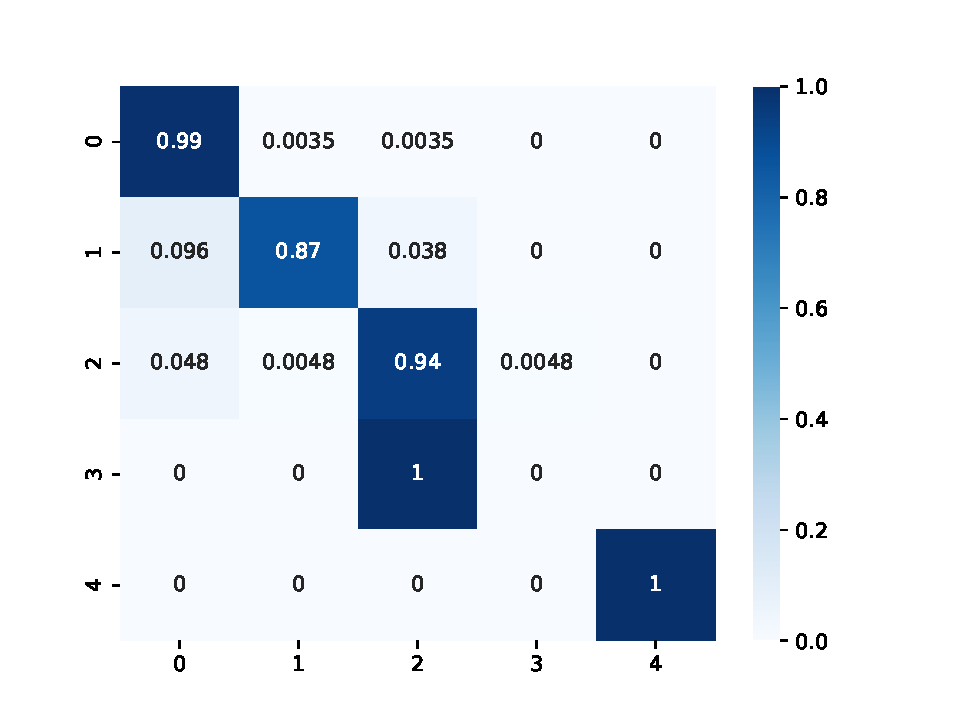
\includegraphics[keepaspectratio, scale=0.3]{images/deep_conv_heatmap.pdf}
        \caption{変更前}
      \end{minipage}
      \begin{minipage}[b]{0.45\linewidth}
        \centering
        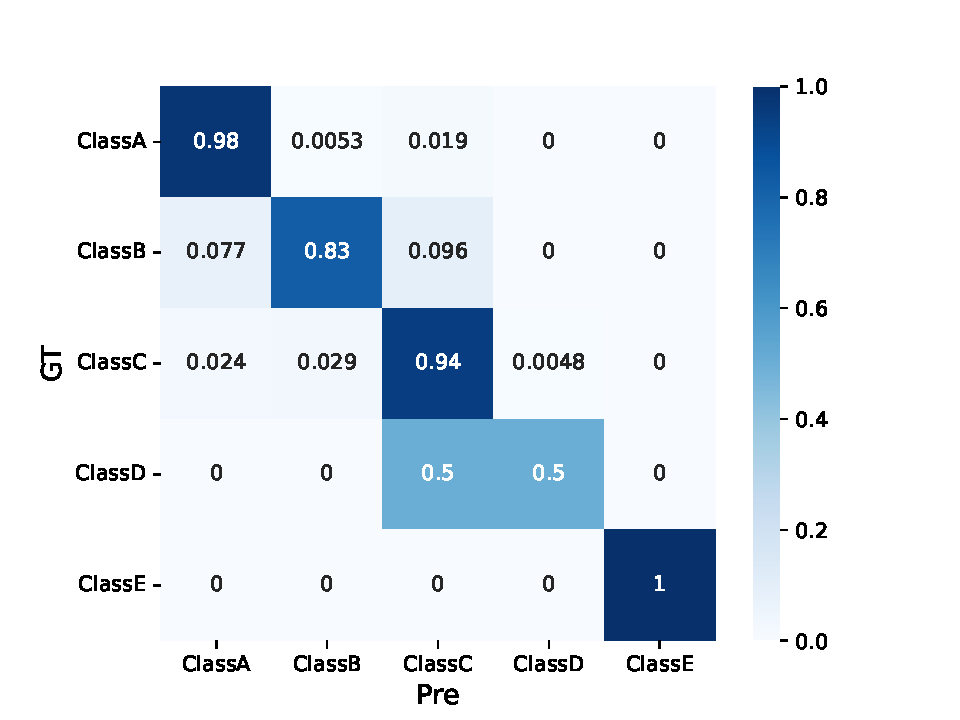
\includegraphics[keepaspectratio, scale=0.3]{images/deepimfam_confusion_matrix_ratio.pdf}
        \caption{変更後}
      \end{minipage}
    \end{figure}
  \end{frame}

  \begin{frame}{これからやること}
    \begin{itemize}
      \item F値の計算
    \end{itemize}
  \end{frame}

\end{document}


